\documentclass[tikz,border=8pt]{standalone}
% Shared look for every TikZ diagram. Load with \input{../../tools/tikz-style.tex}
\usepackage[T1]{fontenc}
\usepackage{lmodern}
\renewcommand{\sfdefault}{lmr}  % diagrams use the same serif as the text
\usetikzlibrary{arrows.meta, positioning, shapes.geometric, calc, fit, backgrounds}
\definecolor{cblue}{HTML}{4C78A8}
\definecolor{corange}{HTML}{F58518}
\definecolor{cgreen}{HTML}{54A24B}
\definecolor{cred}{HTML}{E45756}
\definecolor{cpurple}{HTML}{B279A2}
\definecolor{cgrey}{HTML}{6B6B6B}
\tikzset{
  every picture/.style={font=\sffamily, line width=1.2pt},
  box/.style={draw=#1, fill=#1!12, rounded corners=4pt, align=center, inner sep=7pt, minimum height=1.1cm},
  box/.default=cgrey,
  arrow/.style={-{Stealth[length=3mm]}, draw=cgrey, line width=1.4pt},
  title/.style={font=\sffamily\bfseries\Large},
  note/.style={font=\sffamily\small, text=cgrey, align=center},
}
\AtBeginDocument{\hyphenpenalty=10000 \exhyphenpenalty=10000}

\begin{document}
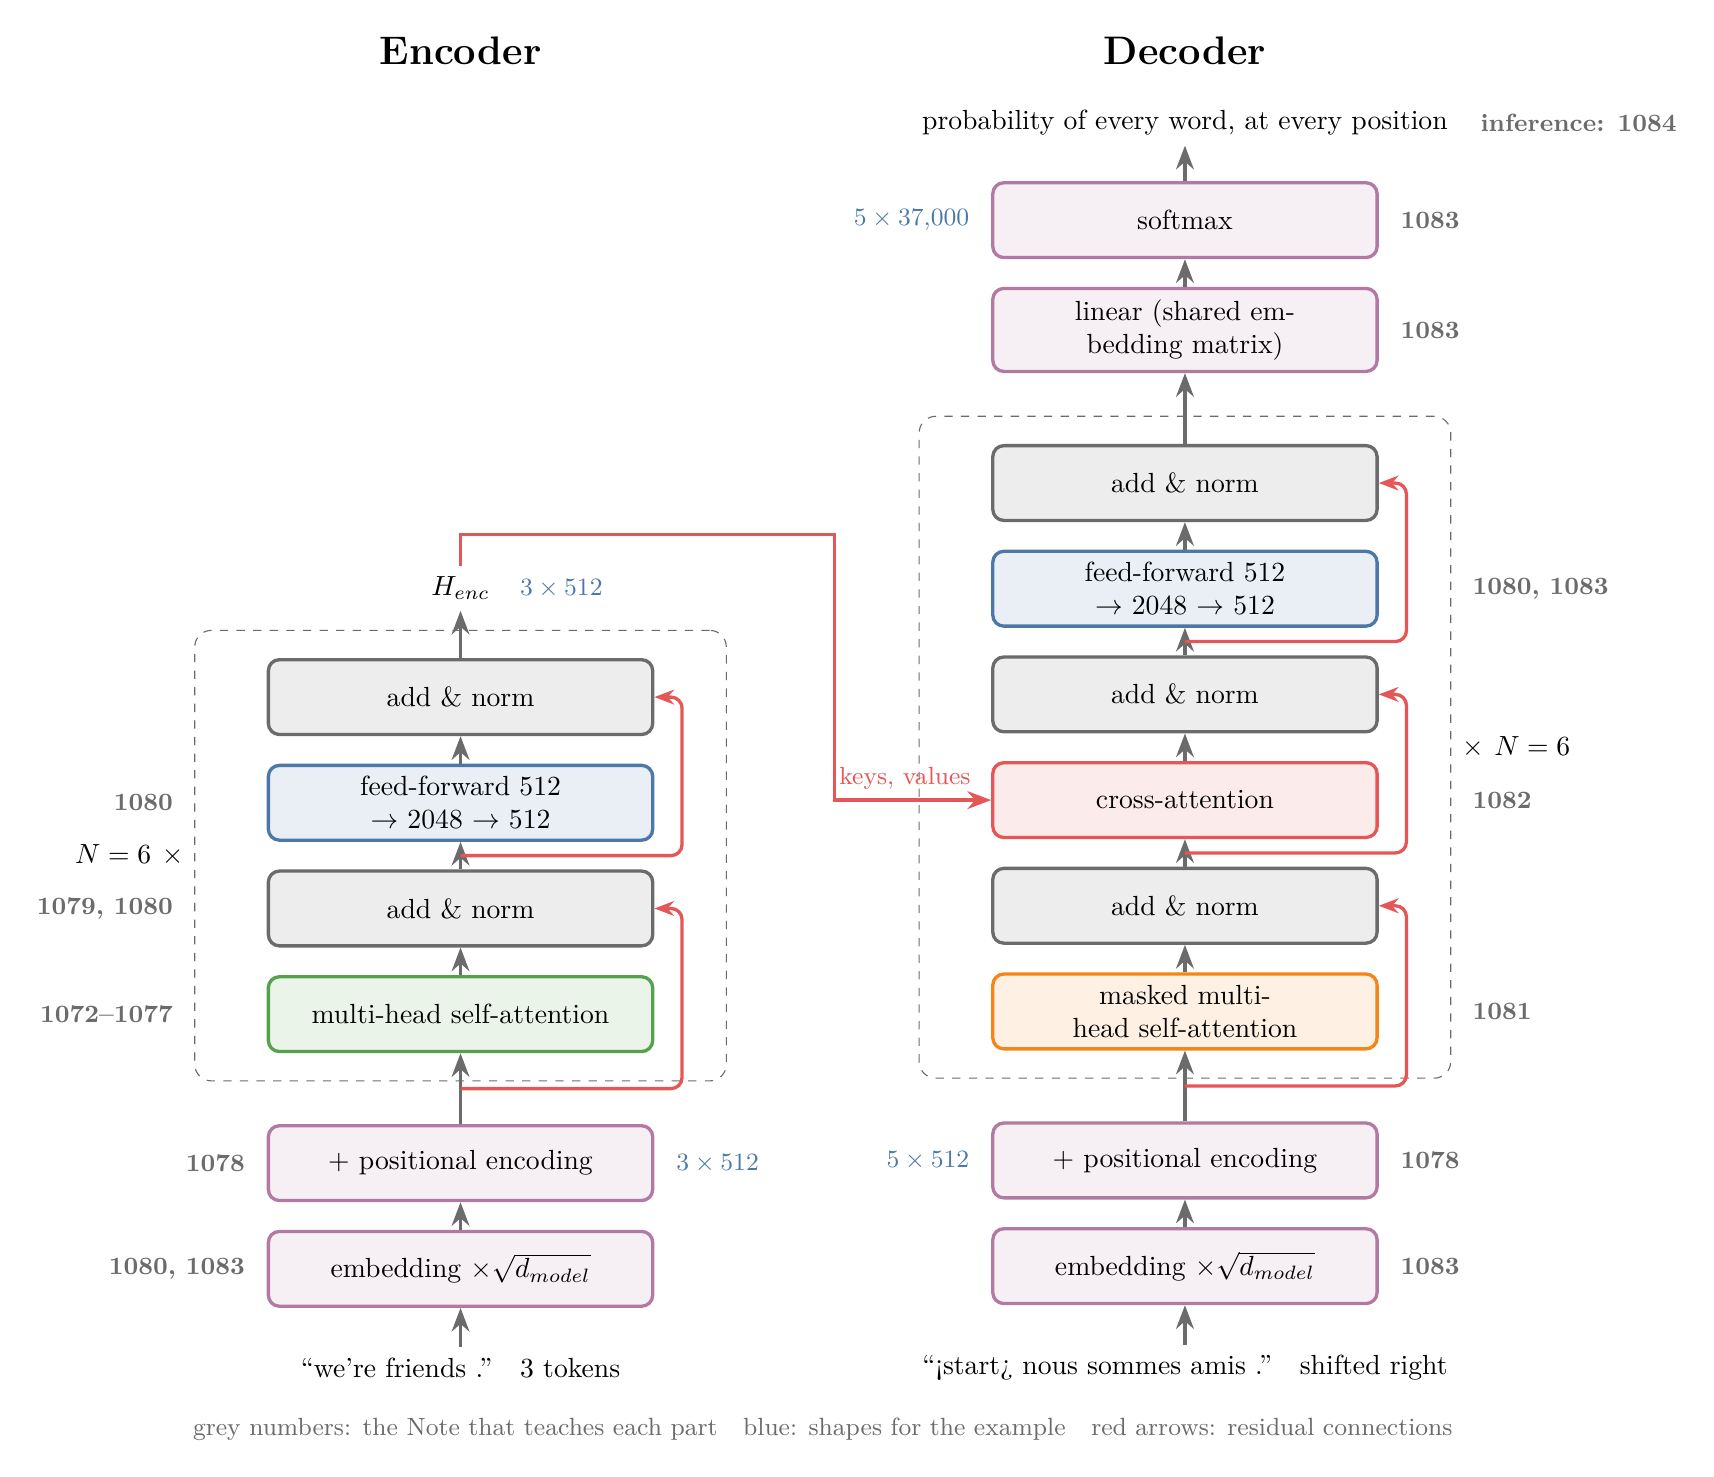
\begin{tikzpicture}[
  part/.style={box=#1, text width=4.6cm, minimum height=0.95cm, inner sep=4pt, font=\sffamily},
  nn/.style={font=\sffamily\small\bfseries, text=cgrey},
  shp/.style={font=\sffamily\small, text=cblue},
  res/.style={-{Stealth[length=2.5mm]}, draw=cred, line width=1.2pt, rounded corners=4pt}]
  % ---------------- encoder ----------------
  \node[font=\sffamily] (ein) at (0, 0) {``we're friends .''\quad 3 tokens};
  \node[part=cpurple, above=0.5cm of ein] (eemb) {embedding $\times\sqrt{d_{\text{model}}}$};
  \node[part=cpurple, above=0.35cm of eemb] (epe) {$+$ positional encoding};
  \node[part=cgreen, above=0.9cm of epe] (emha) {multi-head self-attention};
  \node[part=cgrey, above=0.35cm of emha] (ean1) {add \& norm};
  \node[part=cblue, above=0.35cm of ean1] (effn) {feed-forward 512 $\to$ 2048 $\to$ 512};
  \node[part=cgrey, above=0.35cm of effn] (ean2) {add \& norm};
  \begin{scope}[on background layer]
    \node[draw=cgrey, dashed, rounded corners=6pt, fit=(emha)(ean2), inner xsep=26pt, inner ysep=10pt] (eblk) {};
  \end{scope}
  \node[font=\sffamily\bfseries, anchor=east] at (eblk.west) {$N = 6\ \times$};
  \node[font=\sffamily, above=0.6cm of ean2] (henc) {$H_{\text{enc}}$};
  \foreach \a/\b in {ein/eemb, eemb/epe, epe/emha, emha/ean1, ean1/effn, effn/ean2, ean2/henc} \draw[arrow] (\a) -- (\b);
  \draw[res] ($(epe.north)!0.5!(emha.south)$) -| ([xshift=10pt]emha.east) |- (ean1.east);
  \draw[res] ($(ean1.north)!0.5!(effn.south)$) -| ([xshift=10pt]effn.east) |- (ean2.east);
  % ---------------- decoder ----------------
  \node[font=\sffamily] (din) at (9.2, 0) {``<start> nous sommes amis .''\quad shifted right};
  \node[part=cpurple, above=0.5cm of din] (demb) {embedding $\times\sqrt{d_{\text{model}}}$};
  \node[part=cpurple, above=0.35cm of demb] (dpe) {$+$ positional encoding};
  \node[part=corange, above=0.9cm of dpe] (dmask) {masked multi-head self-attention};
  \node[part=cgrey, above=0.35cm of dmask] (dan1) {add \& norm};
  \node[part=cred, above=0.35cm of dan1] (dcross) {cross-attention};
  \node[part=cgrey, above=0.35cm of dcross] (dan2) {add \& norm};
  \node[part=cblue, above=0.35cm of dan2] (dffn) {feed-forward 512 $\to$ 2048 $\to$ 512};
  \node[part=cgrey, above=0.35cm of dffn] (dan3) {add \& norm};
  \begin{scope}[on background layer]
    \node[draw=cgrey, dashed, rounded corners=6pt, fit=(dmask)(dan3), inner xsep=26pt, inner ysep=10pt] (dblk) {};
  \end{scope}
  \node[font=\sffamily\bfseries, anchor=west] at (dblk.east) {$\times\ N = 6$};
  \node[part=cpurple, above=0.9cm of dan3] (lin) {linear (shared embedding matrix)};
  \node[part=cpurple, above=0.35cm of lin] (soft) {softmax};
  \node[font=\sffamily, above=0.45cm of soft] (out) {probability of every word, at every position};
  \foreach \a/\b in {din/demb, demb/dpe, dpe/dmask, dmask/dan1, dan1/dcross, dcross/dan2, dan2/dffn, dffn/dan3, dan3/lin, lin/soft, soft/out} \draw[arrow] (\a) -- (\b);
  \draw[res] ($(dpe.north)!0.5!(dmask.south)$) -| ([xshift=10pt]dmask.east) |- (dan1.east);
  \draw[res] ($(dan1.north)!0.5!(dcross.south)$) -| ([xshift=10pt]dcross.east) |- (dan2.east);
  \draw[res] ($(dan2.north)!0.5!(dffn.south)$) -| ([xshift=10pt]dffn.east) |- (dan3.east);
  % encoder output into every cross-attention
  \coordinate (mid) at (4.75, 0);
  \draw[arrow, draw=cred] (henc.north) -- ++(0, 0.4) -| (mid |- dcross.west) -- node[font=\sffamily\small, text=cred, above, pos=0.45] {keys, values} (dcross.west);
  % Note numbers
  \node[nn, anchor=east] at ([xshift=-4pt]eemb.west) {1080, 1083};
  \node[nn, anchor=east] at ([xshift=-4pt]epe.west) {1078};
  \node[nn, anchor=east] at ([xshift=-30pt]emha.west) {1072--1077};
  \node[nn, anchor=east] at ([xshift=-30pt]ean1.west) {1079, 1080};
  \node[nn, anchor=east] at ([xshift=-30pt]effn.west) {1080};
  \node[nn, anchor=west] at ([xshift=4pt]demb.east) {1083};
  \node[nn, anchor=west] at ([xshift=4pt]dpe.east) {1078};
  \node[nn, anchor=west] at ([xshift=30pt]dmask.east) {1081};
  \node[nn, anchor=west] at ([xshift=30pt]dcross.east) {1082};
  \node[nn, anchor=west] at ([xshift=30pt]dffn.east) {1080, 1083};
  \node[nn, anchor=west] at ([xshift=4pt]lin.east) {1083};
  \node[nn, anchor=west] at ([xshift=4pt]soft.east) {1083};
  \node[nn, anchor=west] at ([xshift=4pt]out.east) {inference: 1084};
  % shapes
  \node[shp, anchor=west] at ([xshift=4pt]epe.east) {$3 \times 512$};
  \node[shp, anchor=west] at (henc.east) {\ $3 \times 512$};
  \node[shp, anchor=east] at ([xshift=-4pt]dpe.west) {$5 \times 512$};
  \node[shp, anchor=east] at ([xshift=-4pt]soft.west) {$5 \times 37{,}000$};
  \node[title, above=0.3cm of henc |- out.north, anchor=south] at (henc |- out.north) {Encoder};
  \node[title, anchor=south] at ([yshift=0.3cm]out.north) {Decoder};
  \node[note, anchor=north] at (4.6, -0.5) {grey numbers: the Note that teaches each part\quad blue: shapes for the example\quad red arrows: residual connections};
\end{tikzpicture}
\end{document}
